\documentclass{beamer}
\usetheme{Madrid}

\usecolortheme{default}
\useinnertheme{circles}
\usepackage[brazilian]{babel}
\usepackage[utf8]{inputenc}
\usepackage{amsmath,mathtools,amsfonts,amssymb}
\usepackage{graphicx}
\usepackage{booktabs}
\usepackage{array}
\usepackage{hyperref}

% Figuras geradas pelo pipeline em confiabilidade/code/resultados/figuras/
\graphicspath{{../../code/resultados/figuras/}}

\title[Confiabilidade Motor-Bomba]{Análise de Confiabilidade de Bombas Centrífugas Industriais Acionadas por Motor Elétrico com Base em Dados Experimentais de Vibração}
\subtitle{EEE017 --- Confiabilidade de Sistemas}
\author[Felipe / Isabella / Stéphanie]{Felipe / Isabella / Stéphanie \\ {\footnotesize Prof. Michel Bessani}}
\institute[UFMG]{Universidade Federal de Minas Gerais}
\date{\today}

\begin{document}

% ===================== CAPA =====================
\begin{frame}
    \titlepage
\end{frame}

% ===================== AGENDA =====================
\begin{frame}{Roteiro}
    \tableofcontents
\end{frame}

% =====================================================================
\section{Os Dados}
% =====================================================================

% Slide: a cara dos dados
\begin{frame}{A cara dos dados: vibração bruta}
    \textbf{Fonte:} conjunto de dados público de \textbf{Bruinsma \textit{et al.} (2024)} --- bancadas motor-bomba centrífuga da Marinha Real Holandesa.
    \vspace{0.2cm}
    \begin{itemize}
        \item Cada arquivo \texttt{.csv} é o sinal de \textbf{um acelerômetro} (em $g$) de \textbf{uma condição}.
        \item Cada coluna numérica (\textbf{0, 1, 2, \ldots, 14}) é uma \textbf{repetição independente} da mesma medição.
    \end{itemize}
    \vspace{0.15cm}
    \footnotesize
    \begin{tabular}{lrrrcr}
        \toprule
        \textbf{time (s)} & \textbf{0} & \textbf{1} & \textbf{2} & $\cdots$ & \textbf{14} \\
        \midrule
        0,00005 & $-0{,}274$ & $-0{,}055$ & $0{,}128$ & $\cdots$ & $0{,}041$ \\
        0,00010 & $0{,}212$ & $-0{,}080$ & $-0{,}185$ & $\cdots$ & $-0{,}033$ \\
        0,00015 & $0{,}078$ & $0{,}143$ & $0{,}009$ & $\cdots$ & $0{,}112$ \\
        \bottomrule
    \end{tabular}
    \normalsize
    \vspace{0.2cm}
    \begin{block}{}
        \texttt{time}: instante em segundos. Colunas $0$ a $14$: os ensaios repetidos da mesma condição (mesmo sensor).
    \end{block}
\end{frame}

% Slide: as 2 bancadas e velocidades
\begin{frame}{Duas bancadas, duas velocidades}
    \begin{columns}
        \column{0.52\textwidth}
        \footnotesize
        \textbf{Motor-2} --- Grundfos MG160MA
        \begin{itemize}
            \item \textbf{4 polos}, 11\,kW (nominal 1480\,RPM).
            \item Pasta ``75'' $=$ \textbf{75\% da velocidade nominal} $\rightarrow$ \textbf{1110\,RPM}.
            \item Modo estudado: \textbf{rolamento (BPFI)}.
        \end{itemize}
        \vspace{0.2cm}
        \textbf{Motor-4} --- Grundfos MG180MB
        \begin{itemize}
            \item \textbf{2 polos}, 22\,kW (nominal 2950\,RPM).
            \item Pasta ``70'' $=$ \textbf{70\% da velocidade nominal} $\rightarrow$ \textbf{2070\,RPM}.
            \item Modos: \textbf{desbalanceamento} (motor/bomba) e \textbf{desalinhamento}.
        \end{itemize}
        \column{0.48\textwidth}
        \begin{block}{Atenção: ``75'' e ``70'' não são Hz}
            \footnotesize São \textbf{percentuais da velocidade nominal}, ajustados pelo inversor (VFD).\\[4pt]
            RPM síncrono $= \dfrac{120\,f}{n^\circ\text{ polos}}$ (onde $f$ é a frequência da rede em Hz)\\[4pt]
            Valores \textbf{medidos} ($\pm 5$\,RPM):\\
            Motor-2 @ 75\% $\rightarrow$ 1110\,RPM\\
            Motor-4 @ 70\% $\rightarrow$ 2070\,RPM
        \end{block}
    \end{columns}
\end{frame}

% Slide: os 4 modos de falha
\begin{frame}{Os quatro modos de falha analisados}
    \footnotesize
    \begin{tabular}{lllcl}
        \toprule
        \textbf{Modo} & \textbf{Bancada} & \textbf{Canal} & \textbf{Banda} & \textbf{Subsistema} \\
        \midrule
        Rolamento (BPFI)        & Motor-2 / 1110\,RPM & ch1 & 1--9\,kHz & motor \\
        Desbal. no motor        & Motor-4 / 2070\,RPM & ch2 & 10--200\,Hz & motor \\
        Desbal. na bomba        & Motor-4 / 2070\,RPM & ch5 & 10--200\,Hz & bomba \\
        Desalinhamento paralelo & Motor-4 / 2070\,RPM & ch1 & 10--300\,Hz & bomba \\
        \bottomrule
    \end{tabular}
    \normalsize
    \vspace{0.2cm}
    \begin{block}{O que são os ``canais''}
        \footnotesize Canais (\textbf{ch1 a ch5}) são os 5 acelerômetros espalhados pela máquina. Para a extração da assinatura, selecionou-se o canal com resposta \textbf{mais sensível} a cada tipo de falha.
    \end{block}
    \vspace{0.1cm}
    \footnotesize
    \begin{itemize}
        \item Canal e banda escolhidos por física e validados por \textbf{Spearman $\geq 0{,}89$} entre indicador e severidade.
    \end{itemize}
\end{frame}

% Slide: frequencia de amostragem
\begin{frame}{Frequência de amostragem e duração}
    \begin{columns}
        \column{0.55\textwidth}
        \begin{itemize}
            \item Taxa de amostragem: \textbf{20\,kHz} (20.000 amostras/s, passo de 50\,$\mu$s).
            \item Cada arquivo: \textbf{$\sim$240.000 linhas}.
            \item $\dfrac{240{.}000}{20{.}000} = \mathbf{12\ \text{segundos}}$ de sinal por medição.
        \end{itemize}
        \column{0.45\textwidth}
        \begin{alertblock}{Ponto crucial}
            O dataset \textbf{não é \textit{run-to-failure}}.\\[4pt]
            São \textbf{\textit{snapshots}}: fotografias de 12\,s da máquina em diferentes níveis de severidade --- \textbf{não} há eixo de tempo de vida real.
        \end{alertblock}
    \end{columns}
    \vspace{0.2cm}
    \footnotesize Consequência: ninguém ``mediu'' quando a máquina falhou. O tempo até a falha precisa ser \textbf{construído por modelagem} (ver adiante).
\end{frame}

% =====================================================================
\section{Estrutura dos Dados}
% =====================================================================

% Slide: estrutura de pastas
\begin{frame}[fragile]{Estrutura de pastas e o que os nomes significam}
\footnotesize
\normalsize
    \begin{tabular}{ll}
        \toprule
        \textbf{Pasta} & \textbf{Significado} \\
        \midrule
        \texttt{healthy 1,2,3} & baseline saudável (nível 0) --- 3 repetições \\
        \texttt{bearing bpfi 1} & defeito de rolamento --- \textbf{severidade 1} (leve) \\
        \texttt{bearing bpfi 2} & defeito de rolamento --- \textbf{severidade 2} \\
        \texttt{bearing bpfi 3} & defeito de rolamento --- \textbf{severidade 3} (severa) \\
        \bottomrule
    \end{tabular}
    \vspace{0.2cm}
    \begin{itemize}
        \item \texttt{healthy} $=$ nível 0; severidades $=$ níveis 1, 2, 3, \dots
    \end{itemize}
\end{frame}

% Slide: tabela original vs gerada
\begin{frame}{De 28 tabelas gigantes a uma tabela de 958 linhas}
    \footnotesize
    \textbf{Entrada:} \textbf{28 arquivos} \texttt{.csv} (4 modos: \textit{healthy} + severidades). Cada um tem \textbf{240.000 linhas} (12\,s $\times$ 20\,kHz) e \textbf{várias colunas} (repetições).
    \vspace{0.1cm}

    \begin{block}{O papel dos 20\,kHz e a extração do valor RMS}
        Cada coluna (ensaio de $12$\,s com $240.000$ amostras) fornece excelente \textbf{resolução espectral}. Esse sinal no tempo é convertido para o \textbf{domínio da frequência} \textit{(utilizando Análise de Envelope e FFT)}.\\[3pt]
        A energia é filtrada e integrada apenas nas frequências do defeito. O \textbf{valor RMS final} não é a vibração global, mas sim a \textbf{energia concentrada especificamente no modo de falha} para aquele ensaio. Assim, condensamos $240.000$ linhas de um ensaio em um único número, totalizando $958$ indicadores.
    \end{block}
    \vspace{0.1cm}
    \textbf{Saída (\texttt{features.csv}) --- formato longo:} cada linha $=$ uma repetição.
    \vspace{0.05cm}

    \begin{tabular}{llrr}
        \toprule
        \textbf{modo} & \textbf{condicao} & \textbf{nivel} & \textbf{valor (RMS)} \\
        \midrule
        bpfi & healthy 1      & 0 & 0,431 \\
        bpfi & healthy 1      & 0 & 0,428 \\
        bpfi & bearing bpfi 1 & 1 & 0,472 \\
        bpfi & bearing bpfi 3 & 3 & 0,571 \\
        \bottomrule
    \end{tabular}
    \hfill {\scriptsize $240.000 \times 28 \approx 6{,}7$ M de amostras}
    \normalsize
\end{frame}

% =====================================================================
\section{Metodologia}
% =====================================================================

% Slide: features so para media e limites
\begin{frame}{Passo 1--2: as \textit{features} fixam o ``mapa'' da degradação}
    \begin{columns}
        \column{0.52\textwidth}
        \footnotesize
        \textbf{Glossário:}
        \begin{itemize}
            \item \textbf{\textit{Baseline}} ($\mu_0$): vibração média da máquina \textbf{saudável} (nível 0). É o ponto de partida.
            \item \textbf{Sev} (severidade): cada nível de defeito induzido (sev 1, 2, 3\dots). $D_{\max}$ é a \textbf{média de todas as vibrações} da severidade mais alta (sev 3), representando o topo da falha observada no ensaio.
            \item \textbf{Limiar de falha} ($L$): valor de vibração que define falha (``quebrou''). O fator $0{,}5$ coloca a máquina na zona de alerta baseando-se em normativas como a ISO 10816, ficando no \textbf{meio} entre saudável e pior sev:
            $$L = \mu_0 + 0{,}5\,(D_{\max}-\mu_0).$$
        \end{itemize}
        {\tiny \textbf{As \textit{features} N\~{A}O viram tempo!!!}}
        \column{0.48\textwidth}
        \begin{center}
            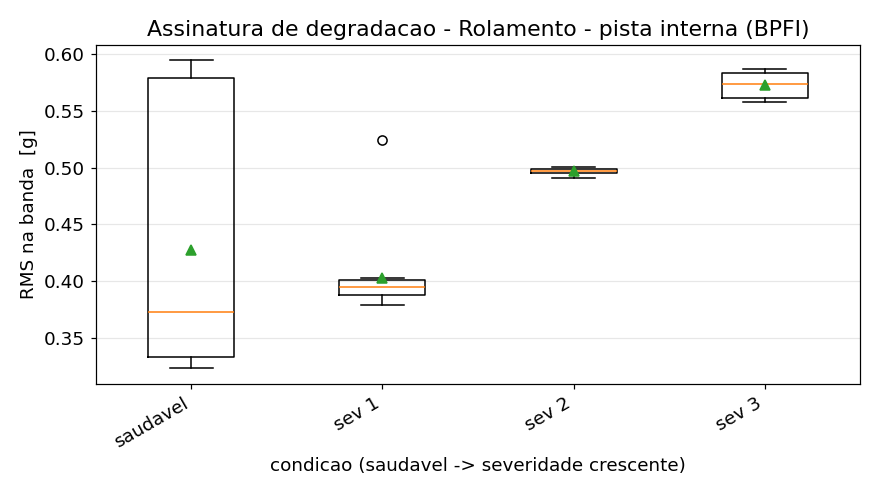
\includegraphics[width=\linewidth]{p1_assinatura_bpfi.png}
        \end{center}
        \footnotesize A vibração (RMS) sobe de forma monotônica do \textit{baseline} até a severidade máxima: é a ``assinatura'' da degradação.
    \end{columns}
\end{frame}

% Slide: geracao dos TTF
\begin{frame}{Passo 2: como os TTF são gerados}
    \begin{columns}
        \column{0.46\textwidth}
        \footnotesize
        \textbf{1) Severidade $\rightarrow$ tempo (hipótese):} cada nível ``acontece'' a cada \textbf{1.000\,h}.
        \vspace{0.1cm}

        \begin{tabular}{ll}
            \toprule
            \textbf{Nível} & \textbf{Tempo ($\tau$)} \\
            \midrule
            saudável & 0\,h \\
            sev 1 & 1.000\,h \\
            sev 2 & 2.000\,h \\
            sev 3 & 3.000\,h $=\tau_{\max}$ \\
            \bottomrule
        \end{tabular}
        \vspace{0.1cm}

        \textbf{2) Curva:} $D(\tau)=D_0\,e^{\rho\tau}$, taxa média $\bar\rho = \dfrac{\ln(D_{\max}/\mu_0)}{\tau_{\max}}$. $\tau$ vai de $0$ a $3000$\,h. $\rho$ é a taxa individual sorteada; $\bar\rho$ é a média do lote \textit{(o gráfico ilustrando esta curva exponencial é mostrado no próximo slide)}.
        \column{0.54\textwidth}
        \footnotesize
        \textbf{3) Monte Carlo --- 2.000 ``cópias''.} Cada unidade recebe:
        \begin{itemize}
            \item $D_0$ sorteado dos valores saudáveis reais;
            \item taxa própria $\rho = \bar\rho \cdot e^{\,\mathcal{N}(0,\,0{,}4)}$ (40\% de dispersão entre unidades);
            \item falha quando cruza $L$: $\displaystyle t = \frac{\ln(L/D_0)}{\rho}$.
        \end{itemize}
        \begin{block}{Censura à direita}
            \footnotesize Se $t > \tau_{\max}$, a unidade ``sobreviveu'' à janela $\Rightarrow$ \textbf{censurada} (não sabemos quando falha, só que é $> 3000$\,h).
        \end{block}
    \end{columns}
\end{frame}

% Slide: exemplo numerico TTF
\begin{frame}{Passo 2: exemplo numérico (rolamento BPFI)}
    \begin{columns}
        \column{0.5\textwidth}
        \footnotesize
        O $D_0$ de cada máquina é \textbf{sorteado} dos ensaios saudáveis reais, e o $\rho$ da normal.\\[4pt]
        $\mu_0 = 0{,}43$; \quad $D_{\max}=0{,}57$; \quad $L = 0{,}50$;\\ $\bar\rho \approx 9{,}4\times10^{-5}$/h; \quad $\tau_{\max}=3000$\,h.
        \vspace{0.2cm}
    
        \scriptsize
        \begin{tabular}{ccrl}
            \toprule
            \textbf{Unidade} & $\rho\,(\times 10^{-5})$ & $t$ (h) & \textbf{status} \\
            \midrule
            \#1 (rápida) & 11,5 & 1727 & falhou cedo \\
            \#2 (médio) & 5,71 & 2641 & falhou \\
            \#3 (lenta) & 2,83 & $>$3000 & censurada \\
            \bottomrule
        \end{tabular}
        \footnotesize
        \column{0.5\textwidth}
        \begin{center}
            \includegraphics[width=\linewidth]{../../code/exemplo_curva.png}
        \end{center}
    \end{columns}
    \vspace{0.25cm}

    \textbf{Tabela gerada (\texttt{ttf.csv}):}
    \footnotesize
    \begin{tabular}{lrr}
        \toprule
        \textbf{modo} & \textbf{ttf} & \textbf{censura} \\
        \midrule
        bpfi & 1727 & 0 \\
        bpfi & 2641 & 0 \\
        bpfi & 3000 & 1 \\
        \bottomrule
    \end{tabular}
    \normalsize
    \hfill\footnotesize $\Rightarrow$ 2.000 linhas por modo.
\end{frame}

% Slide: histograma TTF
\begin{frame}{Passo 2: distribuição empírica dos TTF}
    \begin{columns}
        \column{0.55\textwidth}
        \begin{center}
            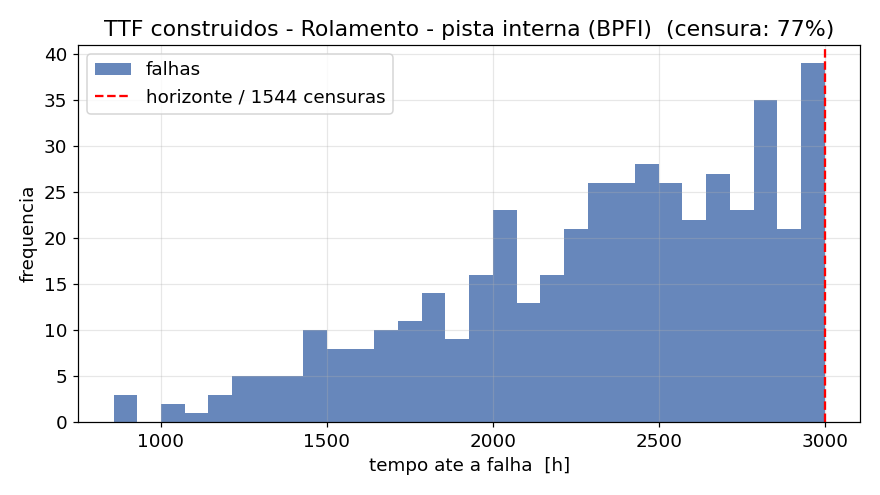
\includegraphics[width=\linewidth]{p2_ttf_bpfi.png}
        \end{center}
        \column{0.45\textwidth}
        \begin{itemize}
            \item A \textbf{variabilidade de 40\%} transforma uma rampa única em uma \textbf{distribuição de vidas}.
            \item Sem ela, todas as unidades falhariam no mesmo instante.
            \item Alta censura (ex: 77\% no BPFI) indica componente \textbf{robusto} que não cruza o limiar em 3000\,h.
        \end{itemize}
    \end{columns}
\end{frame}

% Slide: ajuste de distribuicoes
\begin{frame}{Passo 3: ajuste de distribuições de vida}
    \begin{columns}
        \column{0.5\textwidth}
        \small
        Sobre os 2.000 TTF (gerados com base nos estados de sev 1, 2, 3 e saudável), ajusta-se por \textbf{máxima verossimilhança}:
        \vspace{-0.1cm}
        \begin{itemize}\setlength{\itemsep}{0pt}\setlength{\parskip}{0pt}
            \item \textbf{Exponencial} ($\lambda$ taxa constante);
            \item \textbf{Weibull} ($\beta$ forma/declive, $\eta$ escala/vida útil);
            \item \textbf{Lognormal} ($\mu$ média log, $\sigma$ desvio log).
        \end{itemize}
        \vspace{0.05cm}
        \begin{block}{O que é o AICc e a CDF}
            \scriptsize \textbf{AICc} (\textit{Akaike Information Criterion corrected}) mede o \textbf{ajuste} penalizando o nº de parâmetros. \textbf{Menor vence.}\\Fórmula*: $AICc = 2k - 2\ln(\hat{L}) + \frac{2k(k+1)}{n-k-1}$\\
            {\tiny *Critério proposto por Hirotugu Akaike (1974), versão corrigida por Sugiura (1978).}\\[2pt]
            \textbf{CDF} (\textit{Cumulative Distribution Function}): probabilidade acumulada de falha até o tempo $t$.
        \end{block}
        \column{0.5\textwidth}
        \begin{center}
            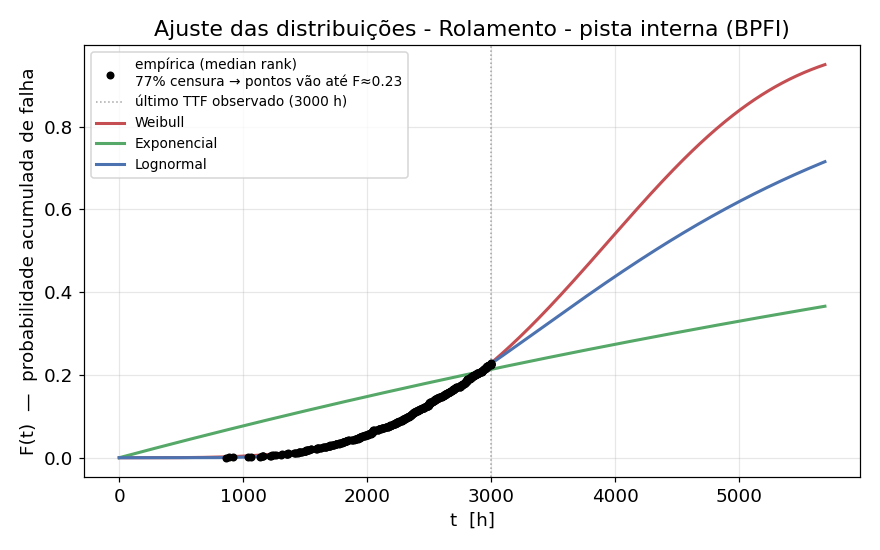
\includegraphics[width=\linewidth]{p3_cdf_bpfi.png}
        \end{center}
        \footnotesize Ajuste das três CDFs aos \textit{median ranks} (método de Benard com correção de censura).
    \end{columns}
\end{frame}

% Slide: tabela parametros e vencedora
\begin{frame}{Passo 3: parâmetros e distribuição vencedora}
    \scriptsize
    \begin{tabular}{lcccc}
        \toprule
        \textbf{Modo} & \textbf{Melhor} & $\beta$ & $\eta$ (h) & \textbf{AICc (W / E / L)} \\
        \midrule
        Rolamento (BPFI) \textbf{(M2)} & \textbf{Lognormal} & 3,82 & 4270 & 8944 / 9516 / \textbf{8935} \\
        Desbal. motor \textbf{(M4)}    & \textbf{Lognormal} & 0,98 & 4567 & 26449 / 26452 / \textbf{26180} \\
        Desbal. bomba \textbf{(M4)}    & \textbf{Lognormal} & 1,68 & 1914 & 28840 / 29384 / \textbf{28757} \\
        Desalinhamento \textbf{(M4)}   & \textbf{Lognormal} & 2,92 & 3096 & 29219 / 31087 / \textbf{29099} \\
        \bottomrule
    \end{tabular}
    \vspace{0.1cm}
    \begin{block}{Por que a Lognormal vence? E por que usar a Weibull?}
        \scriptsize A \textbf{Lognormal} vence (menor AICc) porque a degradação multiplicativa ($D=D_0 e^{\rho\tau}$) gera matematicamente vidas log-normais. Contudo, adotamos a \textbf{Weibull} para os índices (MTTF, Disp., $R(t)$, $\beta$ na curva da banheira). O $\eta$ é o tempo em que $\approx 63\%$ falham.
    \end{block}
\end{frame}


% Slide: bootstrap
\begin{frame}{Passo 4: intervalos de confiança por \textit{bootstrap}}
    \begin{columns}
        \column{0.5\textwidth}
        \small
        \begin{itemize}
            \item Reamostra os TTF com reposição ($r=10^4$ iterações garantem a convergência do intervalo de confiança).
            \item Reajusta a Weibull em cada reamostra, pois foi o método definido na literatura (fornece \textbf{$\beta$} = comportamento da falha e \textbf{$\eta$} = tempo característico).
            \item Percentis 2,5\% e 97,5\% $\Rightarrow$ \textbf{IC 95\%} de $\beta$ e $\eta$.
        \end{itemize}
        \vspace{0.2cm}
        \footnotesize Esta banda de confiança empírica é a única \textbf{legítima} pois não pressupõe normalidade dos parâmetros, sendo usada no gráfico final de $R(t)$ (Confiabilidade).
        \column{0.5\textwidth}
        \begin{center}
            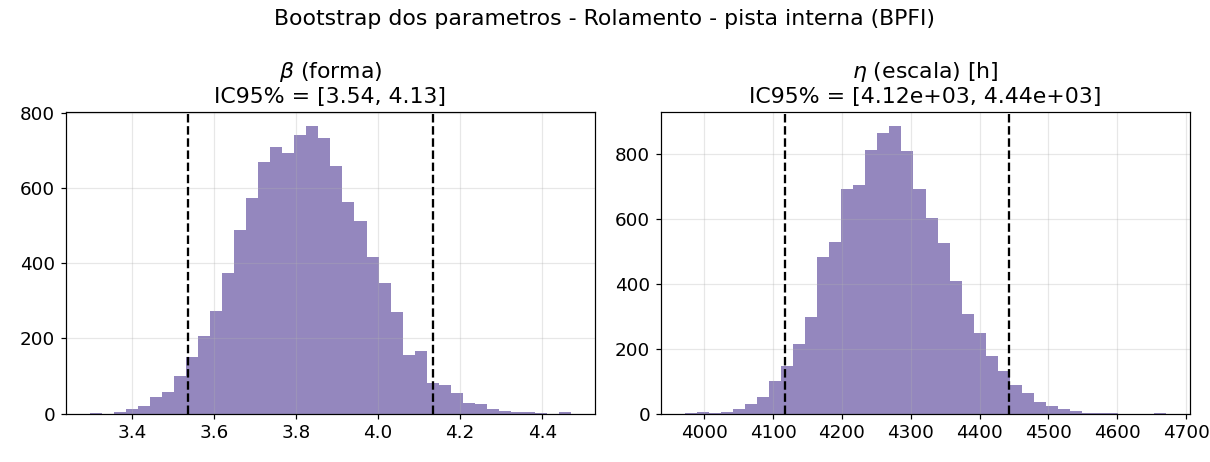
\includegraphics[width=\linewidth]{p4_bootstrap_bpfi.png}\\[0.2cm]
            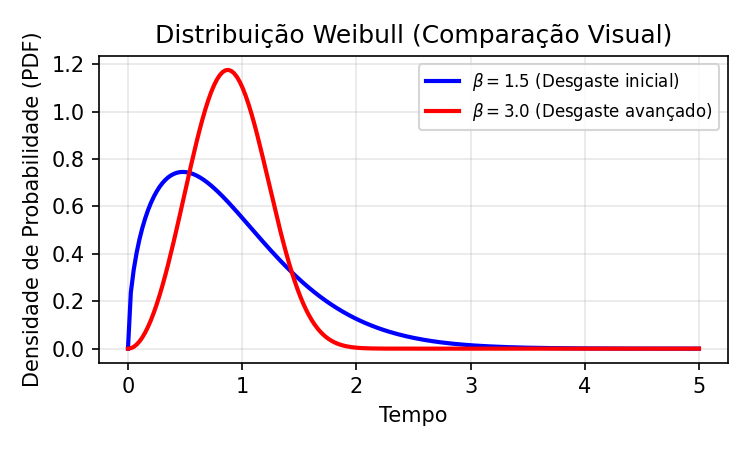
\includegraphics[width=0.7\linewidth]{weibull_generica.png}
        \end{center}
    \end{columns}
\end{frame}

% =====================================================================
\section{Índices de Confiabilidade}
% =====================================================================

% Slide: indices finais
\begin{frame}{Passo 5: índices finais de confiabilidade}
    \footnotesize
    \begin{tabular}{lrcl}
        \toprule
        \textbf{Modo} & \textbf{MTTF (h)} & \textbf{Disponibilidade} & \textbf{Estágio ($\beta$)} \\
        \midrule
        Rolamento (BPFI) \textbf{(M2)} & 4857 & 0,99508 & desgaste ($\beta{=}3{,}82$) \\
        Desbal. motor \textbf{(M4)}    & 5997 & 0,99601 & $\sim$constante ($\beta{=}0{,}98$)* \\
        Desbal. bomba \textbf{(M4)}    & 1836 & 0,98710 & desgaste ($\beta{=}1{,}68$) \\
        Desalinhamento \textbf{(M4)}   & 2831 & 0,99159 & desgaste ($\beta{=}2{,}92$) \\
        \bottomrule
    \end{tabular}
    \scriptsize
    \vspace{0.2cm}
    \begin{itemize}
        \item \textit{MTTF} (Mean Time To Failure) $=$ valor esperado (média matemática) da distribuição Weibull ajustada;\\ \textit{MTTR} (Mean Time To Repair) $=24$\,h (tempo médio de reparo);\\ \textit{A} (Disponibilidade) $= \dfrac{\textit{MTTF}}{\textit{MTTF}+\textit{MTTR}}$.
        \item *O Desbalanceamento no motor resultou em $\beta \approx 1$ indicando taxa de falha constante (típico de eventos aleatórios na vida útil). A bomba é o elo mais fraco.
    \end{itemize}
\end{frame}

% Slide: R(t), h(t), banheira
\begin{frame}{Passo 5: $R(t)$, $h(t)$ e curva da banheira}
    \begin{columns}
        \column{0.5\textwidth}
        \begin{center}
            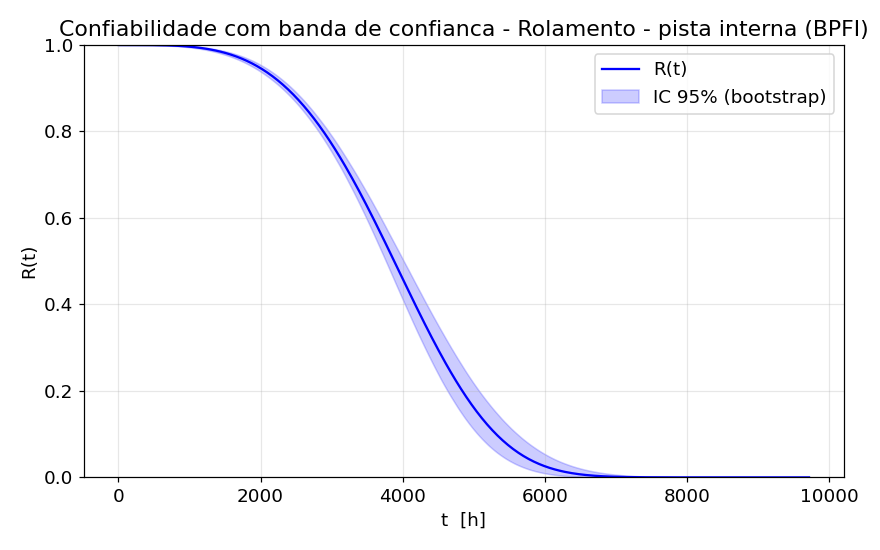
\includegraphics[width=\linewidth]{p5_R_banda_bpfi.png}\\[2pt]
            \footnotesize $R(t)$ com banda de confiança \textit{bootstrap}.
        \end{center}
        \column{0.5\textwidth}
        \begin{center}
            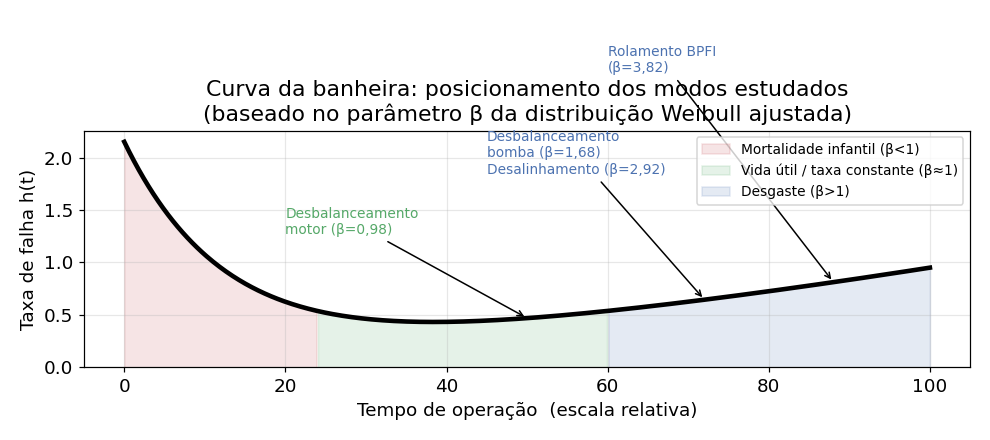
\includegraphics[width=\linewidth]{curva_banheira.png}\\[2pt]
            \footnotesize $\beta$ localiza cada modo na curva da banheira.
        \end{center}
    \end{columns}
\end{frame}

% =====================================================================
\section{Modelo de Sistema}
% =====================================================================



% Slide: monte carlo do sistema
\begin{frame}{Passo 6: modelo do sistema (Monte Carlo)}
    \small
    Neste passo usamos os modelos do motor M4 (que acopla a bomba) para criar um conjunto \textbf{motor em série com a bomba} (a falha de um derruba o conjunto). Simulam-se 3 arquiteturas para comparar como redundâncias afetam o sistema M4:
    \vspace{0.15cm}
    \begin{itemize}
        \item \textbf{Série:} um conjunto ativo. \hfill $t = \min(t_{\text{motor}}, t_{\text{bomba}})$
        \item \textbf{Paralelo:} dois conjuntos ativos, basta um. \hfill $t = \max(t_A, t_B)$
        \item \textbf{Standby (reserva fria):} reserva entra após a 1ª falha. \hfill $t = t_A + t_B$
    \end{itemize}
    \vspace{0.15cm}
    \begin{block}{Disponibilidade verificada analiticamente}
        Série: $A=A_m A_b$;\quad Paralelo: $1-(1-A)^2$;\\
        Standby: $\dfrac{\mu^2+\mu\lambda}{\mu^2+\mu\lambda+\lambda^2}$ (Cadeia de Markov: $\lambda$ é a taxa de falha e $\mu$ é a taxa de reparo).
    \end{block}
\end{frame}

% Slide: resultados do sistema
\begin{frame}{Passo 6: resultados do sistema}
    \begin{columns}
        \column{0.48\textwidth}
        \scriptsize
        \begin{tabular}{lcc}
            \toprule
            \textbf{Config.} & \textbf{Disp.} & $R(2000\,\text{h})$ \\
            \midrule
            Série    & 0,98316 & 0,191 \\
            Paralelo & 0,99972 & 0,348 \\
            Standby  & 0,99970 & \textbf{0,642} \\
            \bottomrule
        \end{tabular}
        \vspace{0.2cm}
        \begin{itemize}
            \item MTTF do conjunto único na bancada real (série) $\approx \mathbf{1369}$\,h.
            \item Analisou-se $R(2000\,\text{h})$ (sobrevivência até 2.000h) como \textbf{missão} ilustrativa dentro da janela de 3000h. Note que Standby aumenta enormemente as chances de cumprir essa missão.
            \item A Disponibilidade do Paralelo é ligeiramente maior porque não há tempo de "partida" da reserva.
        \end{itemize}
        \column{0.52\textwidth}
        \begin{center}
            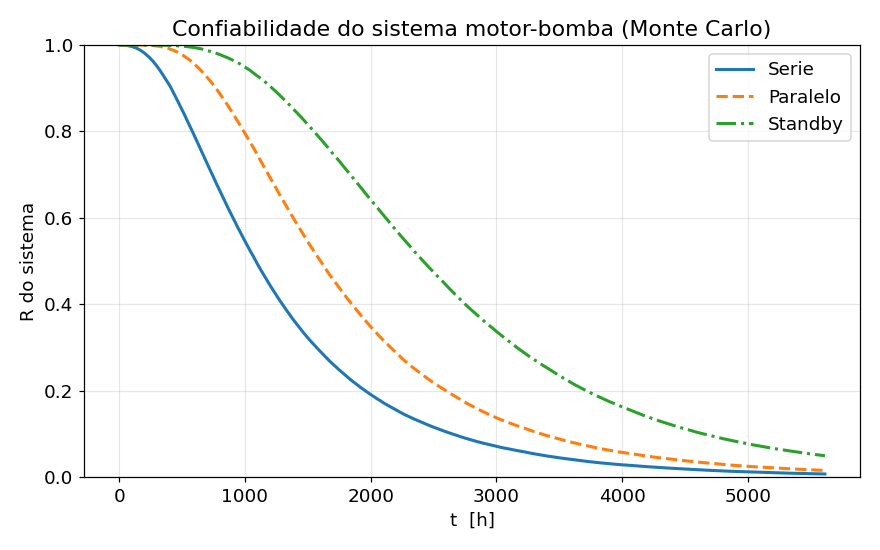
\includegraphics[width=\linewidth]{p6_sistema_R.png}
        \end{center}
    \end{columns}
\end{frame}



\end{document}
